\documentclass[12pt,border=0pt]{standalone}

\usepackage[utf8]{inputenc} 
\usepackage{amssymb,amsmath}
\usepackage{tikz}
\usepackage{color}


\thispagestyle{empty}

\begin{document}

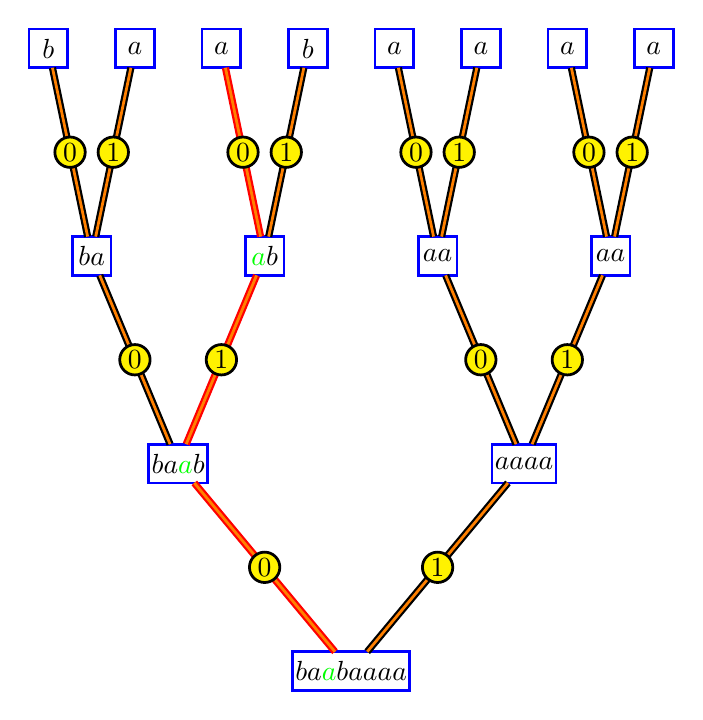
\begin{tikzpicture}[x=5pt,y=6pt]
  \centering
  \tikzset{VertexStyle/.style = {
    shape         = rectangle,
    draw          = blue, 
    fill          = white, 
  	line width    = 1pt, 
    text          = black,
    inner sep     = 1pt,
    outer sep     = 0pt,
    minimum size  = 14 pt,
    scale         = 1
    }
  }
  \tikzset{EdgeStyle/.style = {
    draw            = black, 
    thick,
    double          = orange,
    double distance = 1pt
    }
  }
  \tikzset{EdgeLabelStyle/.style = {
    draw          = black,
  	shape         = circle, 
  	line width    = 1pt, 
  	minimum size  = 10pt, 
    inner sep     = 1pt,
    outer sep     = 0pt,
    fill          = yellow,
    text          = black,
    scale         = 1
    }
  }

	\node[VertexStyle](A1) at (25, 0) {$ba{\color{green}a}baaaa$};
	\node[VertexStyle](B1) at (12.5, 12.5) {$ba{\color{green}a}b$};
	\node[VertexStyle](B2) at (37.5, 12.5) {$aaaa$};
	\node[VertexStyle](C1) at (6.25, 25) {$ba$};
	\node[VertexStyle](C2) at (18.75, 25) {${\color{green}a}b$};
	\node[VertexStyle](C3) at (31.25, 25) {$aa$};
	\node[VertexStyle](C4) at (43.75, 25) {$aa$};
	\node[VertexStyle](D1) at (3.125, 37.5) {$b$};
	\node[VertexStyle](D2) at (9.375, 37.5) {$a$};
	\node[VertexStyle](D3) at (15.625, 37.5) {$a$};
	\node[VertexStyle](D4) at (21.875, 37.5) {$b$};
	\node[VertexStyle](D5) at (28.125, 37.5) {$a$};
	\node[VertexStyle](D6) at (34.375, 37.5) {$a$};
	\node[VertexStyle](D7) at (40.625, 37.5) {$a$};
	\node[VertexStyle](D8) at (46.875, 37.5) {$a$};
	\draw[EdgeStyle, red](A1) to node[EdgeLabelStyle]{$0$} (B1);
	\draw[EdgeStyle](A1) to node[EdgeLabelStyle]{$1$} (B2);
	\draw[EdgeStyle](B1) to node[EdgeLabelStyle]{$0$} (C1);
	\draw[EdgeStyle, red](B1) to node[EdgeLabelStyle]{$1$} (C2);
	\draw[EdgeStyle](B2) to node[EdgeLabelStyle]{$0$} (C3);
	\draw[EdgeStyle](B2) to node[EdgeLabelStyle]{$1$} (C4);
	\draw[EdgeStyle](C1) to node[EdgeLabelStyle]{$0$} (D1);
	\draw[EdgeStyle](C1) to node[EdgeLabelStyle]{$1$} (D2);
	\draw[EdgeStyle, red](C2) to node[EdgeLabelStyle]{$0$} (D3);
	\draw[EdgeStyle](C2) to node[EdgeLabelStyle]{$1$} (D4);
	\draw[EdgeStyle](C3) to node[EdgeLabelStyle]{$0$} (D5);
	\draw[EdgeStyle](C3) to node[EdgeLabelStyle]{$1$} (D6);
	\draw[EdgeStyle](C4) to node[EdgeLabelStyle]{$0$} (D7);
	\draw[EdgeStyle](C4) to node[EdgeLabelStyle]{$1$} (D8);

  \end{tikzpicture}

\end{document}
